
%%%%%%%%%%%%%%%%%%%%%%%%%%%%%%%%%%%%%%%%%%%%%%%%%%%%%%%%%%%%%%
% HUMANOIDS VERSION
%%%%%%%%%%%%%%%%%%%%%%%%%%%%%%%%%%%%%%%%%%%%%%%%%%%%%%%%%%%%%%
\documentclass[conference]{IEEEtran}
% \documentclass[conference]{../sty/IEEEtran}
\IEEEoverridecommandlockouts 
\usepackage{cite}
\usepackage[cmex10]{amsmath}
\usepackage{algorithmic}
\usepackage{array}
\usepackage{mdwmath}
\usepackage{mdwtab}
\usepackage{eqparbox}
\usepackage[tight,footnotesize]{subfigure}
\usepackage[caption=false,font=footnotesize]{subfig}
\usepackage{fixltx2e}
\usepackage{stfloats}
\usepackage{graphicx}
\usepackage{subfigure}
\usepackage{url}

\hyphenation{op-tical net-works semi-conduc-tor}

% *********************************************************
% Math characters shortcuts
\newcommand{\Jps}{ \ensuremath{J^{\dagger}} }
\newcommand{\dx}{ \ensuremath{\dot{x}} }
\newcommand{\dt}{ \ensuremath{\dot{\theta}} }

 
\begin{document}

% *********************************************************
% Paper Info
\title{Redundancy Resolution using Backtracking and Nullspace Search}
\author{Ana Huam\'an Quispe and Mike Stilman% <-this % stops a space
  \thanks{The authors are with the Center for Robotics and Intelligent
    Machines at the Georgia Institute of Technology, Atlanta, GA
    30332, USA. {\tt\small ahuaman3@gatech.edu}, {\tt\small mstilman@cc.gatech.edu}}}
\maketitle

% *********************************************************
\begin{abstract}
%\boldmath
Redundant manipulators pose a non-trivial inverse kinematics problem.
Due to computability restrictions, most of the existing approaches only offer
local optimality guarantees. Most of these methods are based on the nullspace 
projection of the Jacobian and in the Motion Rate control approach introduced 
by Whitney in \cite{Whitney-motionRate-1969}. In this paper, we present a method that also exploits
the nullspace, but instead of projecting arbitrary configurations, we discretize
the nullspace and perform a search, selecting the configuration that maximizes
an optimization function. Additionaly, our algorithm use a backtracking schema 
to escape of local minima. Simulated experiments show that our algorithm solve
problems that cannot be solved otherwise by using a simple Motion Rate Control approach.
We present results with diverse robotic manipulators of up to 9 DOF.  
\end{abstract}

% **********************************************************
\section{Introduction}
Redundancy is a desirable feature in robotic manipulators. The 
additional degrees of freedom allow the robot to not only achieve
its primary goal, such as tracking, but 
it also endows the system with multiple ways to execute the same 
task successfully. Diverse uses of redundancy include obstacle 
avoidance in cluttered environments, control of joint velocities,
avoidance of singularities, etc.

Although redundancy is advantageous, it comes at a
 cost. The complexity of the manipulator increases, which means
that the solution of the inverse kinematics problem does not have
a closed-form solution except for simple or known configurations.
Multiple approaches have been proposed, most of them tailored to
solve the problem under specific assumptions and assessing different
success criteria \cite{hooper-ns-1995}. 

The present paper focuses on solving the most commonly encountered
situation in daily life: To track a task space path
such that it avoids collisions in a static
environment. We present a brief overview of the current work on the area in section 
\ref{sec:RelatedWork}. Section \ref{sec:Overview} gives a general overview of
the inverse kinematics problem and based on it we will explain our
approach on section \ref{sec:ProposedAlgorithm}. We present the 
results of a serie of simulated experiments in section \ref{sec:Experiments}
and end the paper with conclusions and future work in section \ref{sec:Conclusions}.

% ...............................................
% Cover Figure
\begin{figure}[]
  \centering
  \subfigure[Workspace Trajectory]{
    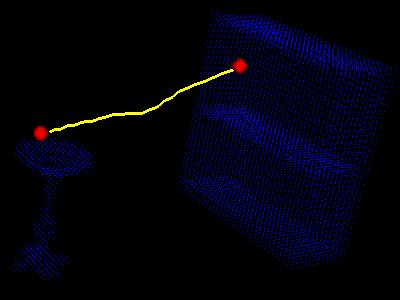
\includegraphics[height=100pt]{figures/Workspace_Path_Barret_1.png} 	
  }
  \subfigure[Execution]{
    \includegraphics[height=100pt]{figures/mosaicImg_Barret_1.png} 
  } 
  \caption{ Experiment with a 7-DOF Barret Arm}
  \label{fig:CoverFigure}
\end{figure}


% ***********************************************************
\section{Related Work}
\label{sec:RelatedWork}
The redundance resolution problem has been vastly studied, being the
pioneering work of Whitney in \emph{Motion Rate Control} (\cite{Whitney-motionRate-1969}) perhaps one of the most influentials in all the methods proposed later. 
Whitney proposed the use of the \emph{Jacobian pseudoinverse} to obtain
solutions that minimized the energy spent. Variations of it included   
Other authors, such as \cite{liegeois-ns-1977} proposed to use
secondary goal functions to achieve.

An excellent overview of these methods can be found in \cite{siciliano-ns-1990}

% *********************************************************
\section{Overview}
\label{sec:Overview}

% ---------------------------------------------------------
\subsection{The Inverse Kinematic Problem}
Given a manipulator with $n$ degrees of freedom and a task that
can be represented by $x$. The direct mapping:

\begin{equation}
x = f(\theta) 
\label{eq:DK}
\end{equation}

\begin{equation}
\dt = \Jps \dx + (I - \Jps J)^{-1}\dot{q}_{0}
\label{eq:IK_MinNorm_Solution}
\end{equation}



% *********************************************************
\section{Proposed Algorithm}
\label{sec:ProposedAlgorithm}


% *********************************************************
\section{Experiments and Results}
\label{sec:Experiments}


% *********************************************************
\section{Conclusions and Future Work}
\label{sec:Conclusions}


% *********************************************************
\section*{Acknowledgments}
The authors would like to thank all members of the Humanoid Lab
at Georgia Tech for their insightful feedback.

% *********************************************************
%\IEEEtriggeratref{8}
%\IEEEtriggercmd{\enlargethispage{-5in}}
\bibliographystyle{IEEEtran}
\bibliography{JnsReferences}


\end{document}


